% ================================================================
% The Retrieve and Connect version of latex/starters/targeted/KS4/geometry/trigBearingsStarter01_workedSolutions.tex
%
% This is the same deck as the one above, made by renaming the titles in it.
% Every slide that was a numbered starter is now titled
% "Retrieve and Connect", and the word is renamed wherever else a title
% used it. Nothing outside a title has been changed.
%
%   made from           latex/starters/targeted/KS4/geometry/trigBearingsStarter01_workedSolutions.tex
%   retitling rules     version 1
%
% Please don't edit this file. It is written again from the one it was
% made from whenever that changes, so an edit here would be lost - edit
% that file instead and this one follows.
% ================================================================
% Root file used ashow macros
\documentclass[aspectratio=169]{beamer}
\usepackage{amsmath}
\usepackage{tikz}
\usetikzlibrary{angles,quotes,calc}

% ================================================================
% Answer-overlay helpers
% ================================================================
\newcommand{\ablank}[1]{%
  \alt<2>{\textcolor{red}{#1}}{\underline{\phantom{#1}}}%
}
\newcommand{\ashow}[1]{\uncover<2->{\textcolor{red}{\small #1}}}
\newcommand{\ashowq}[1]{\alt<2->{\textcolor{red}{\small #1}}{?}}

% Answers drawn straight on to a TikZ diagram, revealed on overlay 2 like \ashow.
% Space is reserved on overlay 1, so the diagram does not move between slides.
\usetikzlibrary{overlay-beamer-styles}
\tikzset{
  ans/.style     = {red, thick, visible on=<2->},
  ansfill/.style = {red!15, visible on=<2->},
  anslab/.style  = {red, font=\tiny, visible on=<2->},
}

\title{Retrieve and Connect}
\author{}
\date{}

\setbeamertemplate{navigation symbols}{}

\begin{document}

\frame{\titlepage}

\begin{frame}{Contents}
\small
\begin{columns}[T]
  \begin{column}{0.5\textwidth}
    \textbf{Questions and short answers}
    \begin{itemize}
      \item \hyperlink{q-st1}{\beamergotobutton{Retrieve and Connect 1}}
    \end{itemize}
  \end{column}
  \begin{column}{0.5\textwidth}
    \textbf{Worked solutions}
    \begin{itemize}
      \item \hyperlink{work-st1}{\beamergotobutton{Retrieve and Connect 1}}
    \end{itemize}
  \end{column}
\end{columns}
\end{frame}

\begin{frame}
  \frametitle{Retrieve and Connect}
  \hypertarget{q-st1}{}

  \begin{columns}[t,onlytextwidth]

    % ===== LEFT COLUMN =====
    \begin{column}{0.4\textwidth}
      % ------------------ Q1 ------------------
      \textbf{1.}


      \vspace{0.7em}
      Which pairs of cardinal directions (North, South, East, West) meet at right angles?

      \ashow{North and East, North and West, South and East, South and West.}

      % ----- Flexible space -----
      \vfill
      \vspace{3em}

      % ------------------ Q3 ------------------
      \textbf{3.}

      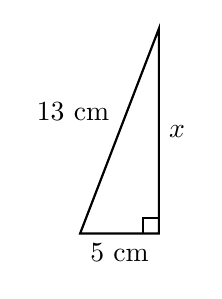
\begin{tikzpicture}[scale=0.2, thick]
        % Right triangle (hypotenuse is 13)
        \coordinate (A) at (0,0);
        \coordinate (B) at (5,0);
        \coordinate (C) at (5,13);

        % Triangle
        \draw (A) -- (B) -- (C) -- cycle;

        % Right angle marker
        \draw ($(B)+(0,1)$) -- ($(B)+(-1,1)$) -- ($(B)+(-1,0)$);

        % Side lengths
        \node[below] at ($(A)!0.5!(B)$) {$5$ cm};
        \node[right] at ($(B)!0.5!(C)$) {$x$};
        \node[above left] at ($(A)!0.5!(C)$) {$13$ cm};

      \end{tikzpicture}

      \vspace{0.5em}
      Find the missing side.

      \ashow{$x = 12$ cm}

    \end{column}

    % ===== RIGHT COLUMN =====
    \begin{column}{0.6\textwidth}
      % ------------------ Q2 ------------------
      
      \textbf{2.}

      \begin{columns}[t,onlytextwidth]
      \begin{column}{0.5\textwidth}

      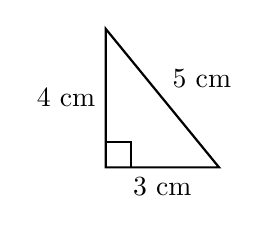
\begin{tikzpicture}[scale=0.8, thick]

        % Coordinates of triangle (hypotenuse longest)
        \coordinate (A) at (0,0);
        \coordinate (B) at (1.8,0);
        \coordinate (C) at (0,2.2);

        % Draw triangle
        \draw (A) -- (B) -- (C) -- cycle;

        % Right angle marker
        \draw ($(A)+(0,0.4)$) -- ($(A)+(0.4,0.4)$) -- ($(A)+(0.4,0)$);

        % Label sides
        \node[below] at ($(A)!0.5!(B)$) {3 cm};
        \node[left]  at ($(A)!0.5!(C)$) {4 cm};
        \node[above right] at ($(B)!0.5!(C)$) {5 cm};

      \end{tikzpicture}
\end{column}
      \begin{column}{0.5\textwidth}
      Which side is the hypotenuse?

      \ashow{The side labelled 5 cm is the hypotenuse.}
\end{column}

    \end{columns}

\textbf{4.}

\begin{columns}[t,onlytextwidth]
  % ===== Diagram Column =====
  \begin{column}{0.45\textwidth}

    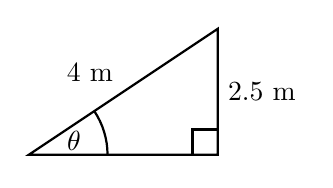
\begin{tikzpicture}[scale=0.8, thick]
      % Triangle for inverse sine
      \coordinate (A) at (0,0);
      \coordinate (B) at (3,0);
      \coordinate (C) at (3,2);

      % Draw triangle
      \draw (A) -- (B) -- (C) -- cycle;

      % Right angle
      \draw ($(B)+(0,0.4)$) -- ($(B)+(-0.4,0.4)$) -- ($(B)+(-0.4,0)$);

      % Side labels
      \node[right] at ($(B)!0.5!(C)$) {$2.5$ m};  % opposite
      \node[above left] at ($(A)!0.5!(C)$) {$4$ m}; % hypotenuse

      % Angle θ at A
      \pic[draw,angle radius=10mm,"$\theta$"{scale=1}] {angle = B--A--C};

    \end{tikzpicture}

  \end{column}

  % ===== Options Column =====
  \begin{column}{0.55\textwidth}

    Find $\theta$.

     \fontsize{10}{12}\selectfont

    \begin{itemize}
        \item[(A)] $\displaystyle \theta = \sin^{-1}\!\left(\frac{2.5}{4}\right)$
        \item[(B)] $\displaystyle \theta = \cos^{-1}\!\left(\frac{2.5}{4}\right)$
        \item[(C)] $\displaystyle \theta = \tan^{-1}\!\left(\frac{2.5}{4}\right)$
    \end{itemize}

    \ashow{Answer: (A)}

  \end{column}
\end{columns}
\end{column}
\end{columns}

\end{frame}

\begin{frame}{Worked Solution: Retrieve and Connect 1, Question 1}
\hypertarget{work-st1}{}

\textbf{Question:} Which pairs of cardinal directions (North, South, East, West) meet at right angles?

\textbf{Worked Solution:}

The cardinal directions are spaced \(90^\circ\) apart around a compass. Two directions meet at a right angle exactly when they are adjacent on the compass, rather than opposite.

The adjacent pairs are:
\[
\text{North and East},\quad \text{North and West},\quad \text{South and East},\quad \text{South and West}.
\]

Thus those four pairs meet at right angles. North and South, and East and West, are straight lines, not right angles.

\end{frame}

\begin{frame}{Worked Solution: Retrieve and Connect 1, Question 2}

\textbf{Question:} In the right-angled triangle with sides \(3\) cm, \(4\) cm and \(5\) cm, which side is the hypotenuse?

\textbf{Worked Solution:}

The hypotenuse is the longest side of a right-angled triangle and is opposite the right angle. Since \(5 > 4 > 3\), the side of length \(5\) cm is the longest; it is opposite the right angle.

Indeed, by Pythagoras:
\[
3^2 + 4^2 = 9 + 16 = 25 = 5^2.
\]

So the hypotenuse is the side labelled \(5\) cm.

\end{frame}

\begin{frame}{Worked Solution: Retrieve and Connect 1, Question 3}

\textbf{Question:} A right-angled triangle has hypotenuse \(13\) cm and one leg \(5\) cm. Find the missing side \(x\).

\textbf{Worked Solution:}

By Pythagoras' theorem,
\[
(\text{hypotenuse})^2 = (\text{leg})^2 + (\text{other leg})^2.
\]

Here the hypotenuse is \(13\) cm and one leg is \(5\) cm, so
\[
13^2 = 5^2 + x^2.
\]

Therefore
\[
169 = 25 + x^2
\]
\[
x^2 = 169 - 25 = 144.
\]

Taking the positive square root, since \(x\) is a length:
\[
x = \sqrt{144} = 12.
\]

\[
\boxed{x = 12\text{ cm}}
\]

\end{frame}

\begin{frame}{Worked Solution: Retrieve and Connect 1, Question 4}

\textbf{Question:} Find \(\theta\) in the right-angled triangle where the side opposite \(\theta\) is \(2.5\) m and the hypotenuse is \(4\) m. The options are:
\[
\text{(A) } \theta = \sin^{-1}\!\left(\frac{2.5}{4}\right),\qquad
\text{(B) } \theta = \cos^{-1}\!\left(\frac{2.5}{4}\right),\qquad
\text{(C) } \theta = \tan^{-1}\!\left(\frac{2.5}{4}\right).
\]

\textbf{Worked Solution:}

In a right-angled triangle,
\[
\sin\theta = \frac{\text{opposite}}{\text{hypotenuse}}.
\]

The side opposite \(\theta\) is \(2.5\) m and the hypotenuse is \(4\) m, so
\[
\sin\theta = \frac{2.5}{4}.
\]

Taking the inverse sine of both sides gives
\[
\theta = \sin^{-1}\!\left(\frac{2.5}{4}\right).
\]

Therefore the correct option is \textbf{(A)}.

\end{frame}

\end{document}